\section{Fault-Injection Framework}
\subsection{Whole-Brain Spiking Substrate}
We adopt the released whole-brain LIF model of \emph{Drosophila} (Section~\ref{sec:introduction}), implemented in Brian2 and built on the FlyWire connectome\cite{lin2024network}. Every neuron is a current-based LIF unit (threshold $-45$\,mV, reset $-52$\,mV, $\tau_m{=}5$\,ms, refractory 2.2\,ms, delay 1.8\,ms). Every chemical synapse is a delta synapse of magnitude $0.275$\,mV signed by the presynaptic cell's neurotransmitter; the connectivity table yields 15{,}091{,}983 edges between 138{,}639 neurons, 40\% of them inhibitory. Global activity is sustained by the released model's calibrated Poisson background drive. Our engine restores the full network state at the start of every trial, so all conditions share identical initial states and background realizations; one 600\,ms trial runs in ${\approx}3.5$\,s on one CPU core.

\subsection{Behavioral Task: Visuomotor Escape}
The instrumented pathway (Fig.~\ref{fig:system}) is the fly's looming-triggered escape circuit: looming-sensitive visual projection neurons LC4 (104) and LPLC2 (210) converge on descending neurons\cite{shuang2023opplod,fu2020complementary}. Because the looming response of these cells contains a sustained high-rate component, we drive them---and, as a control, an equal-sized random neuron set---with independent 150\,Hz Poisson trains through a stimulus layer gated per trial, rather than modeling looming kinetics. The behavioral readout is the population rate of the command set \{DNp01, DNa02, DNp04, DNb01\} (8 neurons) over the last 500\,ms; all 1{,}299 descending neurons serve as a secondary readout. Calibration drove the command population to $94.6$\,Hz (interdecile 93.6--95.8\,Hz, first-spike latency 4.4\,ms on the 10-trial set) under escape stimulation but only 8.2\,Hz (6.4--9.2\,Hz) under random stimulation; we set $\theta=51.4$\,Hz midway between them; every pass/fail classification below is unchanged for any threshold between the distributions' observed trial extremes, 9.2 and 63.1\,Hz. Calibration statistics refer to a 10-trial set; Section~IV baselines use the 12 sweep trials.

\begin{figure}[tb]
\centering
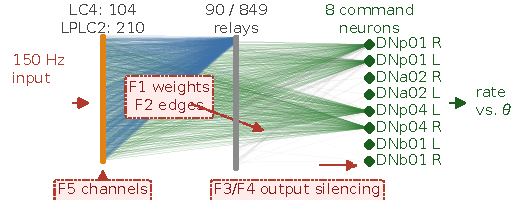
\includegraphics[width=0.96\columnwidth]{figs/fig0_pathway.pdf}
\caption{The instrumented escape pathway, drawn from the connectome itself. Left: the 314 driven sensory cells (LC4, LPLC2); center: top-90 of the 849 two-hop relays; right: the 8 command DNs. Line width and opacity scale with synapse count (594 direct sensory$\to$DN edges); dashed red marks the fault-injection points (F5 channels; F1/F2 synapses; F3/F4 units). Inset: reconstructed adult brain, adapted from Dorkenwald et al.\cite{dorkenwald2024neuronal} (CC~BY~4.0).}
\label{fig:system}
\end{figure}

\subsection{Fault Taxonomy}
Five fault families cover the hardware-relevant failure modes. F1 multiplies every synaptic weight by an i.i.d.\ lognormal factor ($\sigma\in\{0.05,0.1,0.2,0.5\}$), modeling analog weight variability and bit-level imprecision. F2 deletes a random fraction $f\in\{0.05,0.10,0.25,0.50\}$ of synapses, modeling interconnect or memristor failures. F3 silences all output synapses of a random fraction $f\in\{0.01,0.02,0.05,0.10\}$ of units, excluding input and readout cells (equivalent to unit removal in this delta-synapse model), modeling dead cores. F4 applies the same operation to the top 1\%, 2\%, or 5\% of units ranked by total outgoing synapse count (again excluding input and readout), modeling failure of high-fanout components; these cells carry 9--22\% of all synapses (for the 1\%, 2\% and 5\% sets, respectively), so F4 is a targeted, correlated version of F3. F5 zeroes all outgoing synapses of one (LC4 or LPLC2) or both sensory channels, modeling sensor or afferent-path failure. All faults are applied after state restoration and held fixed across the 12 trials of a condition, with SHA-256--derived deterministic realizations.\footnote{Code, connectome-derived edge lists, and per-trial records: \url{https://github.com/Scophield/drosophila-fault-injection}.}

\subsection{Controls}
Two controls isolate what the biological wiring contributes. The first is an ER null: permuting the postsynaptic endpoint of every synapse preserves out-degree, weight, and sign but destroys in-degree structure and convergence motifs; the identical sweep runs on it. The second is analytic: for both graphs we compute the \emph{pathway mass} $m_k=\lVert A^k\rVert_1$ on the input-to-command submatrix ($A$ holds synapse counts, i.e., absolute values of the signed connection strengths), the synapse-weighted mass of $k$-hop directed routes from LC4$\cup$LPLC2 into the descending set, on the intact graph and after the F2 edge-deletion levels; comparing its decay with the simulated behavioral decay separates topological redundancy from dynamical amplification.

